
%%%%%%%%%%%%%%%%%%%%%%%%%%%%%%%%%%%%%%%%%%%%%%
\logvartrue
\chapter{A shared toolbox}
%%%%%%%%%%%%%%%%%%%%%%%%%%%%%%%%%%%%%%%%%%%%%%
\label{chap:alpha}

\section{Common genetic basis for bacterial association with plants}
The plant-bacteria association is indeed a complex interaction, with many possible mechanisms, each one with distinct effects on plant physiology and agriculture (see section \ref{atale2cities}). The various kinds of plant association (endophytism, symbiosis, pathogenicity) are found in many bacterial taxa, with some well-documented examples of bacterial species able to exhibit more than one distinct kind of association with plants \cite{bashan2004azospirillum} \cite{chi2005ascending}; the most studied phylum of bacteria associated with plants belongs to the \textit{Proteobacteria} phylum, with the classes of \textit{alpha}, \textit{beta} and \textit{gamma}-\textit{proteobacteria} as the most studied, especially for the symbiotic nitrogen fixing phenotype. Given the high variability in the association phenotypes and the different mechanisms and signals exchanged, the genetic determinants of such complex interactions are most likely a vast repertoire of many genes, many of which may be not shared across the various taxonomical entities able to interact with plants. Understanding if a common shared set of genetic elements for the interaction with plants exists inside the bacterial kingdom is crucial for both evolutionary and functional studies: on the evolutionary perspective, the origin and dynamics of the plant association genotypes may be derived to gain a more precise history of mutualism/symbiosis, both with plants and more generally with higher organisms. The functional perspective, however, is the one that would have the biggest impact on agriculture, because such shared genetic elements will most probably be key factors in the plant interaction mechanism, and may form the basis for genetic engineering experiments to test their specific role in the plant interaction phenotype.

\subsubsection{Comparative genomics of distant species}
When applied on large heterogenic datasets, the comparative genomics analysis becomes more complex: the presence of different evolutionary distances between each genome is challenging for the orthology assessment step, mostly because an higher evolutionary distance often implies a smaller sequence similarity, which may not be detectable by the Blast algorithm \cite{kim2007clustering}. Another problem posed by comparative genomics analysis on heterogenuos datasets is the presence of species that have experienced a strong genomic reduction, such as obligate symbionts and intracellular pathogens; with the relaxation of evolutionary constraints due to the pathogenic or symbiotic lifestyle, many genes are lost to improve the replication efficiency and speed (see for instance \textit{Buchnera aphidicola}, the obligate endosymbiont of aphids \cite{tamas200250}). As a consequence of this genomic reduction, the presence of these genomes would exclude many otherwise conserved genes from the so-called \textit{core} genome: the exclusion of such genomes is therefore a prerequisite for large comparative genomics studies. Being an interesting functional and evolutionary subject for computational experiments, many algorithms have been developed to perform comparative genomics analysis on a large taxonomical scale: such techniques may involve the use of the information on the phylogenetic relationships between each species to tune the homology search cut-offs \cite{rehmsmeier2001phylogenetic} \cite{qian2003detecting} \cite{qian2004performance}, the use of the protein domain content together with sequence similarity \cite{qian2003detecting} \cite{qian2004performance} \cite{hollich2007pfamalyzer} or the relaxation of the homology cut-offs in order to consider all the homology signals, then clusterized to extract the orthologous families \cite{kim2007clustering}.

\newpage
\section{Plant-bacteria association and symbiosis: are there common genetic traits in \textit{Alphaproteobacteria}?}
The plant association phenotype is a common functional feature inside the class \textit{Alphaproteobacteria}, were many species able to interact with plants either through endophytism, symbiosis or pathogenicity can be studied. Even if the genetic elements needed for a successful symbiosis are well-known, little is known about their occurrence in all the alphaproteobacterial tree, as well as little or no information is available regarding the presence and occurrence of genes necessary to establish an endophytic interaction with a plant. A comparative genomics study on 92 genomes belonging to the alphaproteobacterial class has been carried out to highlight the core genome of this taxa, as well as the conserved genetic elements needed for endophytism and symbiosis, if present. The dataset comprises species that are plant symbionts, endophytes or species that are not associated with plants, with the exclusion of obligate pathogens and other species with reduced genomic sizes. Insights on evolutionary dynamics and phylogenetical distribution of this shared genes has also been analyzed and discussed.

\newpage
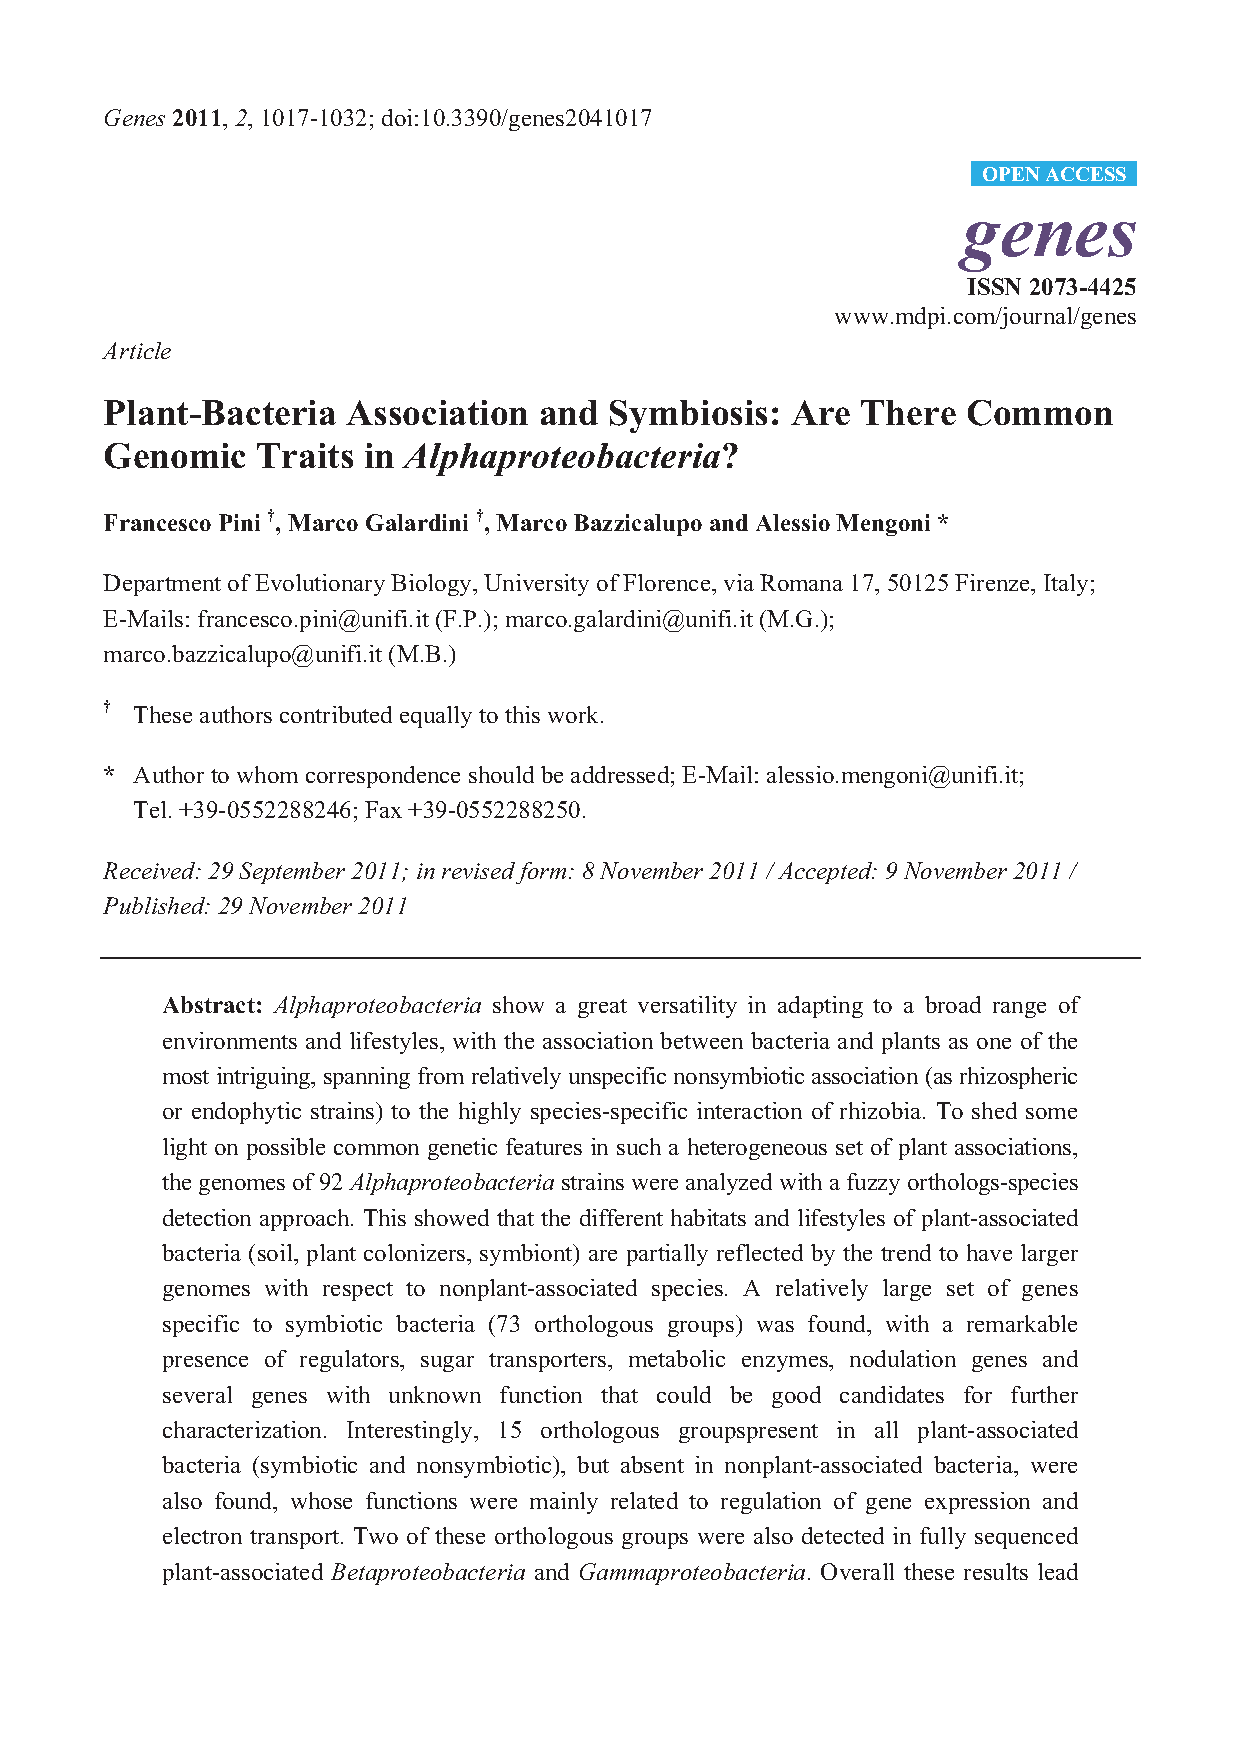
\includepdf[pages=-,offset=10mm 0, scale=0.9]{articles/Pini2011.pdf}
\newpage

%%-----------
%% Backmatter
%%-----------
\backmatter
\chaptermark{Bibliography}
\renewcommand{\sectionmark}[1]{\markright{#1}}
\bibliographystyle{unsrt}                           %Use alpha codes for references
\sectionmark{Bibliography}
\addcontentsline{toc}{chapter}{Bibliography}        %Force addition of Bibliography to TOC    
\bibliography{References}